\documentclass{article} % For LaTeX2e
\usepackage{nips15submit_e,times}
\usepackage{hyperref}
\usepackage{url}
\usepackage{graphicx}
%\documentstyle[nips14submit_09,times,art10]{article} % For LaTeX 2.09

\title{INCAT : Intelligence-based Cybersecurity Awareness Training}
\author{
Tam n. Nguyen, Lydia Sbityakov, Samantha Scoggins\\
North Carolina State University\\
\texttt{\{tam.nguyen, lesbitya, smscoggi\}@ncsu.edu} \\
}
\newcommand{\fix}{\marginpar{FIX}}
\newcommand{\new}{\marginpar{NEW}}
\nipsfinalcopy % Uncomment for camera-ready version
\begin{document}
\maketitle

\begin{abstract}
  The abstract paragraph should be indented  on both the left- and right-hand margins. Use 10~point
  type, with a vertical spacing (leading) of 11~points.  The word
  \textbf{Abstract} must be centered, bold, and in point size 12. Two
  line spaces precede the abstract. The abstract must be limited to
  one paragraph.
\end{abstract}

\section{Introduction}
Cyber security training should be adaptable to evolving cyber threat landscape, be cost effective and most important of all, be integrated well with other components such as enterprise risk management, incident management, threat intelligence and so on. Unfortunately, very few cyber security training platforms can satisfy those requirements.

This paper proposes a new model for conducting cyber security training with three main objectives: (i) training efforts are initiated by emerging relevant threats and delivered first to the most vulnerable groups (ii) each training session must be promptly executed (iii) training results must be able to provide actionable intelligence to be employed by other systems such as enterprise risk management, enterprise threat intelligence, etc.

InCAT stands for "Intelligence-based Cyber Awareness Training" and its feedback loop starts with a threat intelligence feed where the most recent cyber threats will be analyzed. Associated attack vectors (AVs) will be identified. Recent reports from the National Vulnerability Database (NVD) will be parsed and feed into machine learning models to identify the current themes. This angle is called "Technical Severity". From the identified themes, quizzes will be sent to users (samples) within a company (population). Machine learning models will analyze users responses, resulting in a list of vulnerabilities for which employees are least prepared. This angle is called "Human Weakness". Actionable intelligence can be derived from analyzing results gathered from the two angles.

Pedagogical backgrounds are presented in Section 2. High-level design structure and elaborations on our methodologies are presented in Section 3. Implementation details including links to demos, source codes, and sample data are presented in Section 4. Section 5 discusses the current results and our self-critical evaluations of this research project to be followed by Section 6 - "Future works".

\section{Backgrounds}
Human is the weakest link in any cyber defense strategy. 78\% of cyber incidents were caused by careless humans \cite{20172017Overview}. The process of cyber awareness training is full of challenges. First, the threat landscape is evolving rapidly with both internal factors (technology changes, business flows changed, etc) and external factors (changes in supply chain, compliance, competitors, enemies, political climates, etc) \cite{Ingalsbe2008ThreatEnd, Manadhata2011AnMetric}. To make things worst, there is no agile cooperation between cyber awareness education and other departments. 

Second, knowledge is not always translated into correct actions. For example, people who know the types of phishing are not completely immune from actual phishing. Training materials are more focused on teaching the knowledge rather rather the skills of applying the knowledge. Consequently, tests are developed to test just the knowledge, in which case learners are well aware that they are being tested and consciously put their guards on. It is very hard to simulate real world scenarios.

Finally, it is challenging to prepare people for potential unknown threats that have not happened yet, not mentioning cyber adversaries are incredibly creative, sometimes state sponsored.

Abawajy \cite{Abawajy2014UserMethods} did a research on user preference of cyber security awareness methods of text-based, video-based and game-based among 60 participants. Even with a "low-tech" appearance, the performance of text-based education is on par with other "fancy" methods. Employees with work deadlines and projects actually prefer light-weight cyber security awareness delivery method that does not get in the way of their main jobs.

Pawlowski \cite{Pawlowski2016SocialDesign} presented a way to map learners' perceptions toward cyber security topics using data analytics.  Especially of interest for high-impact cyber security training is finding out which topics are either high-interest (may affect individuals personally) or low-awareness (security blind spots) for learners.  Additionally, from a management perspective, how learners can be motivated to continue to learn and stay abreast of new threats is also of high importance.  It was discovered that learners have been exposed to several cyber security key terms and concepts, care very much about cyber security topics that may affect them personally, but that they lack awareness of the bigger picture which also includes national cyber infrastructure and cyber terrorism.

Wei \cite{Wei2017IntegratingAssessment} adopts concept mapping (CM) as a tool to enhance the teaching and evaluating of Information System courses. By analyzing the topology of student CMs, instructors can design CM-based tasks, and grade student CMs against a master CM. While it was not explicitly mentioned in the paper, comparing CM is a very interesting way to identify how the concept map of a student can be changed over time, by education and other factors.

\section{Methodology and Designs}
InCat feedback loop includes 8 main steps as shown in Figure \ref{Figure:IncatDesign}. 

\begin{figure}[h]
  \centering
  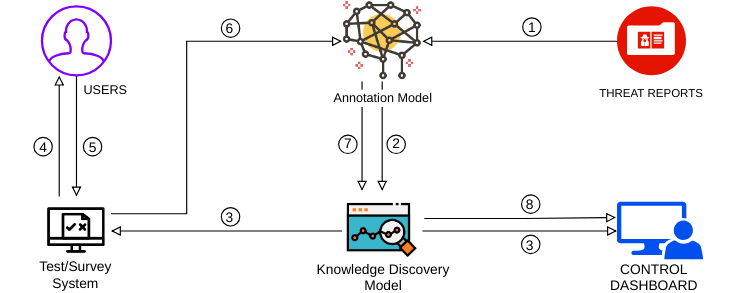
\includegraphics[width=11cm]{images/INCAT-Designs.png}
  \caption{INCAT Design Structure}
  \label{Figure:IncatDesign}
\end{figure}

Threat reports are highly condensed data that relates to cyber threat developments and was prepared by domain experts. Reports will be analyzed by the Annotation Model for identification of key entities and the relationships between them. Newly annotated data will be further analyzed by the Knowledge Discovery Model which will automatically identify newly emerged patterns in cyber threat landscape. The Test/Survey System will construct assessments based on the knowledge components relating to the newly identified patterns and deliver to the users who are most vulnerable. Assessment results will then be returned to the Test/Survey System for initial processing, resulting in reports with scores and users' response texts. Such user assessment reports will be analyzed by the same Annotation Model and the Knowledge Discovery Model. Derived knowledge from threat reports (step 3) and user assessment reports (step 7) are stored in database and be displayed by a Control Dashboard system. Through this dashboard, cyber security analysts may correlate details and derive further actionable intelligence.

\section{Implementation}
\subsection{Data Source and Preprocessing}
The 2018 vulnerability json file, CVE-2018, was downloaded from https://nvd.nist.gov/vuln/data-feeds.  We choose to work with the more updated
Base Metrics 3.0 and used a python program to extract records with completed BM3 fields and convert to a csv file.  Two data sets were then created one for text analysis containing the CVE-ID number and description and the second for clustering containing the ID and remaining categorical fields.  Only the fields of Product and Vendor were sometimes missing and these were imputed to the value of "UNKNOWN" in these cases.  Derivative fields such as baseScore and baseSeverity that were simply calculated from other fields were eliminated from cluster processing.

\subsection{Identifying Attack vectors}
The categorical data set consists of all 6851 available 2018 nvd records with a completed base metric 3 (BM3) section and includes the following features which generally correspond to the vulnerability ontology used in the text analysis (see next section) and based on the NIST17 paper \cite{}: 
\begin{center}
\begin{tabular}{ |l|l| } \hline
Feature & Values\\\hline
Attack Vector & Network, Adjacent, Local, Physical  \\ 
Attack Complexity & Low, High  \\ 
Privileges Required & None, Low, High  \\ 
User Interaction & None, Required  \\ 
Confidentiality Impact & High, Low, None\\
Integrity Impact & High, Low, None\\
Availability Impact & High, Low, None\\
\hline
\end{tabular}
\end{center}


This relatively small set of features and possible values can have 1,296 different combinations.  However, a simple data query reveals that less than 200 combinations contained any threats and 80\% of the vulnerabilities fall into just 16 unique combinations of features. Finding meaningful clusters in the data would help to focus training on the most prevalent threat vectors and make the most efficient use of resources for cyber security training.  

Clustering was used to determine if there was a natural clustering of features and if certain combinations were never seen or exceedingly common. In addition, the features of product and vendor are also available for many records.  Clustering was performed both with and without the additional fields of product and vendor.

Because the data is purely categorical common algorithms such as k-means are not recommended. \cite{}.  DBScan while helpful for removing outliers is not recommended for data with higher dimensions where Euclidean distance is less effective \cite{}.  
Cluster analysis was performed using python and the k-modes module \cite{https://pypi.org/project/kmodes/} \textit{which defines clusters based on the number of matching categories between data points.}   because this package is readily available and specifically designed to work with categorical data.  

\textit{Describe clusters here.
}
The clusters serve to inform the annotation and classification process used in 4.2 and in future could provide the underlying framework for the identification and selection of Attack Vectors on an on-going basis.



\subsection{Annotation Model for Classifying Text Data}
Our data sets of descriptions for Threat Reports were extracted from the National Vulnerability Database which can be considered the gold standard of threat reporting and is being used nation wide. In the form of XML or CSV files, datasets can be imported into Annotation Model which is powered by the IBM Watson Knowledge Studio platform \footnote{https://www.ibm.com/watson/services/knowledge-studio/}.

There are three main steps for building the Annotation Model: (i) Building a system type (ii) Building ground truths by manual annotation (iii) Training and evaluating models.

A system type is a domain-specific ontology enriched with relationships. Since the domain is Cyber Security, we decided to rely on another gold standard - the NIST's recommendations for Cyber Vulnerability Description ontology \cite{Booth2016DraftOntology} which was summarized into Figure \ref{Figure:VulOntology}.

\begin{figure}[h]
  \centering
  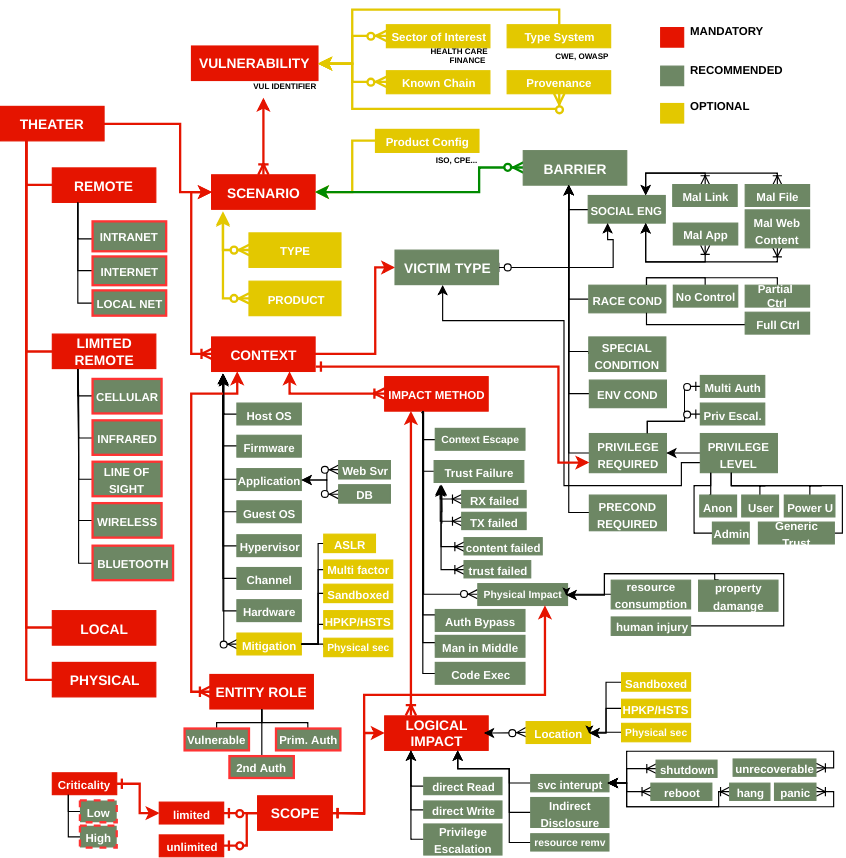
\includegraphics[width=12cm]{images/NISTIR8138.png}
  \caption{Vulnerability Description Ontology}
  \label{Figure:VulOntology}
\end{figure}

It is notable that in real-world scenario, reports will only touch a few "boxes" of this crowded ontology. Therefore, the ontology has to be enriched with relationships that are context-preserving. Such relationships can be described directly by rules or indirectly by type \& sub-type specifications. The novelty of our work comes in the form of our own designed relationship rules, the overloading of the rules and the re-mapped hierarchy of the original NIST's ontology. The detailed description file of our type system (ontology with relationships) can be viewed at our Github repository \footnote{https://github.com/genterist/INCAT-public}. Further elaborations on this type system will be on the final full paper.

In order to build ground truths, we started first with human annotators and manual annotation. Small sets of 50 entries each are extracted from our corpus of 1000 NVD threat reports in 2018. Sets can be specified to have some overlaps in order to support inter-annotation. Team members (except one) will work on their corresponding pre-assigned sets and manually annotate entities together with relationships. At the final step, the one who did not do any manual annotation will go over the results, resolve conflicts and publish annotated entries as ground truths.

On the IBM Watson Knowledge Studio platform, we train and test our models using the manually annotated entries which are separated into training set (70\%), test set(23\%), and blind set(7\%). Training set is used to teach machine the domain specific knowledge through annotated entities and their relationships. Trained model will then perform on test set to produce test set machine results. Upon comparing test set machine results with human annotated results, the accuracy of the model can be defined. Blind set is used to test the system only after several iterations of training and testing. The end result of this process is an annotation model that can be deployed with other models which, in our case, happened to be IBM Knowledge Discovery.

\subsection{Analyzing Users Responses}
The Knowledge Discovery Model is an analytic engine with a front end and a back end. The front end (the Control Dashboard) displays identified patterns, trends and actionable insights using Node.js, React, Semantic UI React, and Chart.js. The back end accepts inputs produced by the annotation model, communicates with IBM Watson Discovery Service API, and renders the views that will be displayed on the front end. The server will also communicate with Qualtrics API in order to initiate the delivery of tests (surveys) to users. The user knowledge testing components will be discussed further in our full paper.

\section{Current Results and Future Works}
At the moment, we have a corpus of over 8000 cyber vulnerability report for 2018 harvested from the National Vulnerability Database (NVD) and 127 user survey entries gathered from a Qualltric-MechanicalTurk campaign. We established a type system and manually annotated 100 entries of NVD corpus and 27 entries of the user survey corpus. It will be slow in the beginning because members who do not have solid backgrounds in cyber security will need more time to annotate cyber threat reports. We are, however, in the process of making over 20 dictionaries covering main entities in our established type system so that in the next few days, machine can help us annotate the key terms in the reports.

A basic dashboard is being built utilizing IBM Watson Knowledge Discovery on top of Watson Knowledge Studio. The near term goals include counting and displaying the counts of relationship types inferred by the AI and ML models. Ultimately, we would like to be able to display inferred statistics from the cyber threat report angle and the user knowledge angle. Please note that these "statistics" are the results of machine models reading and understanding the hidden context behind cyber threat reports and survey takers responses.

%\section{Future works}
%Lorem ipsum

\section{Conclusion}
Our team believes we are on the right schedule to a conference quality paper. We will do further researches to make sure our existing type system is a good one, our human annotated corpus are of high quality with the right quantity, and a good Github repo with carefully documented source codes and data.Due to issues with Overleaf, we had to submit the paper in the state that you have seen. A more detailed, polished version will be readied by appropriate deadline.

\bibliographystyle{IEEEtran}
\bibliography{IEEEabrv,references.bib}

\end{document}